\documentclass[11pt,a4paper]{article}
\usepackage[latin1]{inputenc}
\usepackage[spanish]{babel}
\usepackage{amsmath}
\usepackage{amsfonts}
\usepackage{amssymb}
\usepackage{graphicx}
\usepackage[left=2cm,right=2cm,top=2cm,bottom=2cm]{geometry}
\author{Samuel Caleb Mart�nez Hern�ndez}
\title{Angulos de Euler (Parametrizaci�n)}
\begin{document}

\includegraphics[scale=1]{EV/logo.png} 
\section{Angulos de euler }
\begin{center}
Samuel Caleb Mart�nez Hern�ndez\\ \\
Ing. Mecatr�nica \\ \\
7-A\\ \\
Cinem�tica de Robots\\ \\
\end{center}
\begin{center}
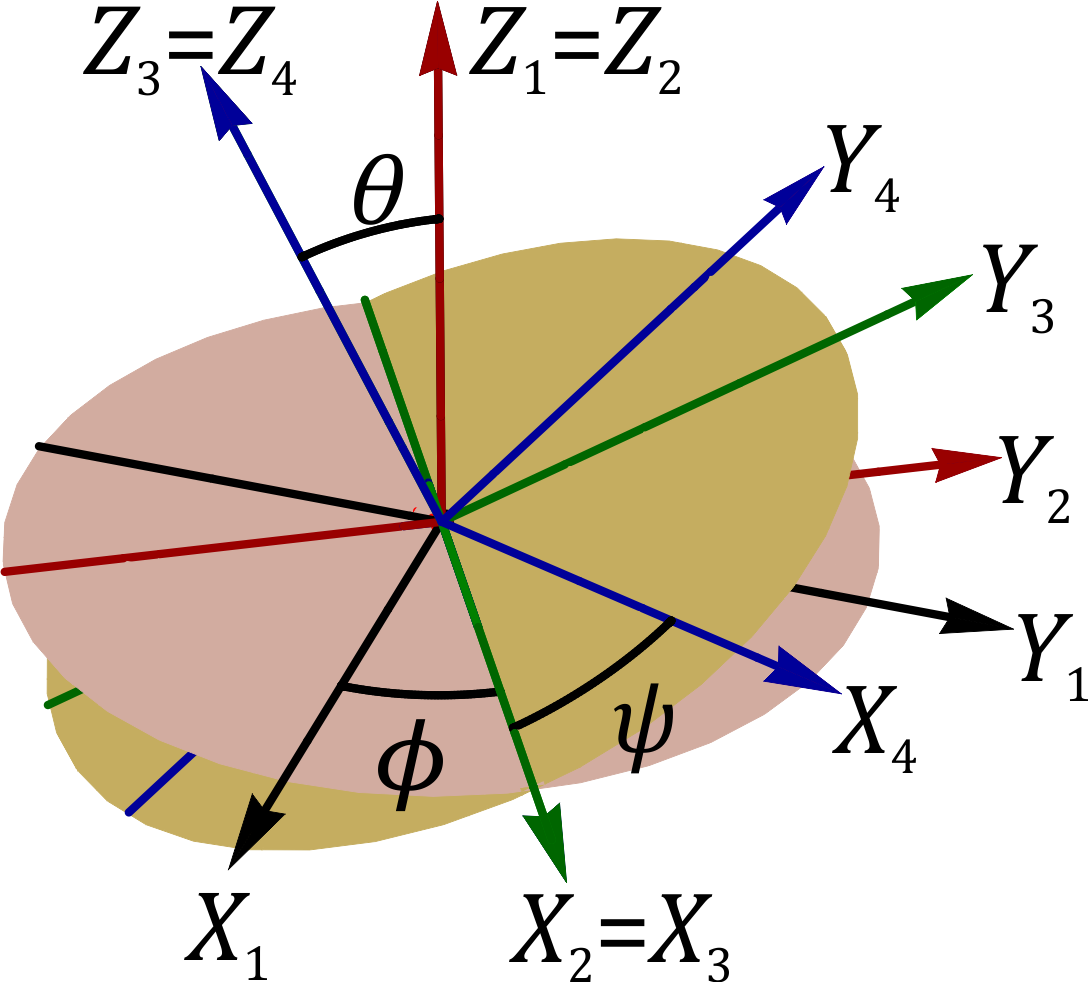
\includegraphics[scale=1]{EV/1.png} 
\end{center}\\ \\

\section{Introducci�n}
Cuando hablamos del tema de los angulos de euler es importante saber una cosa primeramente, si nos referimos al movimiento en general de un cuerpo solido rigido, se sabe que este posee seis grados de libertad, cosa que, en la parametrizacion del movimiento de dicho solido, los seis grados ya mencionados se pueden descomponer en tres de traslaci�n y tres de rotaci�n, estos de un cuerpo respectivamente. \\
\begin{center}
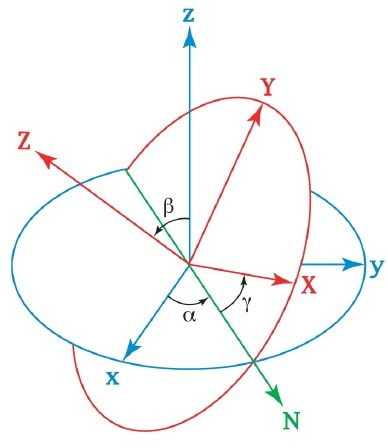
\includegraphics[scale=1]{EV/2.jpg} 
\end{center}\\

Para los grados de libertad de traslaci�n, nos sirve con otorgar el desplazamiento de un punto exacto del solido, es decir, su centro de reducci�n.\\

En cuanto a la rotaci�n, cambian las formas de parametrizarla, haci�ndolas diferentes en si, por as� decirlo, se puede:\\

* Dar la matriz de rotaci�n que pasa de un sistema de referencia ligado al solido, a uno exterior tomado como fijo, dicha matriz cuenta con nueve elementos sometidos a seis v�nculos respectivamente, esto multiplica el numero de ecuaciones que son necesarias para el an�lisis descriptivo del movimiento.\\

*Dar la orientaci�n del eje de giro por medio de dos �ngulos y el �ngulo de giro alrededor de este eje. Cuenta con el inconveniente, como los �ngulos de Euler y otros, que requieren un mucho uso de funciones trigonom�tricas.\\

\section{Posici�n y matriz de rotaci�n}\\

Con el fin de obtener el resultado de la rotaci�n, necesitamos observar qu� posici�n ocupa en el sistema de referencia fijo un punto perteneciente al s�lido. El vector de posici�n se escribir� con componentes diferentes en la base fija y en la base m�vil, aun si se trata del mismo vector.\\
\begin{center}
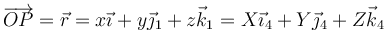
\includegraphics[scale=1]{EV/3.png} 
\end{center}\\
debido a ser un punto del s�lido, las componentes (X,Y,Z) ser�n constantes. El problema radica en que se reduce a relacionar los vectores de las bases. Para ello, componemos las tres rotaciones.\\

La primera rotacion de un angulo tetha en torno a el eje 0z1 = 0z2, que nos lleva al solido 2. La relacion entre la base fija 1 y la intermedia 2, la cual es... \\
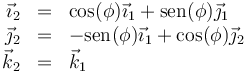
\includegraphics[scale=1]{EV/4.png}\\

Para la inversa se deduce en simples cambios de signo que se acomodan de la siguiente manera... \\  \\
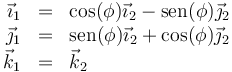
\includegraphics[scale=1]{EV/5.png}\\ \\
 
La segunda rotaci�n se basa en el giro del angulo theta alrededor del eje 0x2=0x3. La linea de nodos de la rotaci�n nos lleva al solido intermedio numero tres, el cual se relaciona directamente con la 2 a causa de....\\ \\
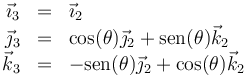
\includegraphics[scale=1]{EV/6.png} \\ \\

Nuevamente, la inversa ...\\ \\ 
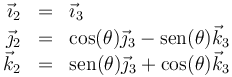
\includegraphics[scale=1]{EV/7.png} \\ \\

Ya para finalizar, el tercer giro el cual corresponde a un nuevo giro de un angulo gama, alrededor del angulo 0z3=0z4 la relaci�n entre las bases 3 y 4 es an�loga a la que hay entre la 1 y la 2.\\ \\
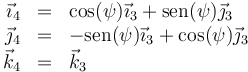
\includegraphics[scale=1]{EV/8.png} \\ \\

Lo mismo, su inversa seria ...\\ \\

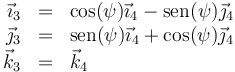
\includegraphics[scale=1]{EV/9.png} \\ \\
Y nuestra matriz de rotaci�n:\\
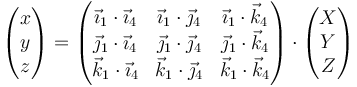
\includegraphics[scale=1]{EV/10.png}\\ \\
 
\section{Conclusi�n}\\
Como idea final de lo que se acaba de realizar, se sabe que la primer rotaci�n es la precesi�n, seguida de la segunda rotaci�n, la nutaci�n y para finalizar con la ultima rotaci�n es decir la tercera, la "rotaci�n". Estas prceden del analisis del movimiento terrestre del solido. La rotaci�n se trato del movimiento alrededor del eje terrestre, la precesi�n es el lento movimiento del eje, el cual provoca que la estrella situada en el polo norte celeste cambie con el pasar del tiempo. Finalmente, la nutaci�n fue el cambio que tuvo el solido en cuanto a la inclinaci�n del eje terrestre. 

\paragraph{Referencias}
@article{gonzalez2008euler,
  title={Euler y la Geometr{\'\i}a Anal{\'\i}tica},
  author={Gonz{\'a}lez Urbaneja, Pedro Miguel},
  journal={Quaderns d'hist{\`o}ria de l'enginyeria},
  volume={9},
  pages={83--116},
  year={2008},
  publisher={Centre de recerca per a la Hist{\`o}ria de la T{\`e}cnica" Francesc Santpon{\c{c}} i Roca~?}
}



\end{document}